\section{Test effettuati} %TODO Graziano, Federica, Carlo i test effettuati da voi
In questa sezione si elencano i test effettuati per il sito in esame.
Per i test di accessibilità eseguiti in remoto, il sito è stato caricato su
GitHub Pages.

\subsection{Validazione XHTML} %DONE
Ogni pagina è stata validata con il tool offerto da W3C all'indirizzo
\texttt{http://validator.w3.org/\#validate\_by\_uri}, con il risultato che
le seguenti pagine non sono valide:
\begin{enumerate}
\item pagina principale del sito;
\item pagina descrittiva di un libro (generata tramite CGI).
\end{enumerate}

\subsection{Validazione CSS} %DONE
Ogni foglio di stile CSS è stato validato con il tool offerto da W3C
all'indirizzo
\texttt{https://jigsaw.w3.org/css-validator/\#validate\_by\_input}, non
trovando alcuna scorrettezza nel codice.

\subsection{Cynthia Says} %DONE
Uno dei tool che è stato utilizzato per l'accessibilità delle pagine è Cynthia
Says, inserendo l'URL di ogni pagina caricata su GitHub Pages e richiedendo la
conformità a WCAG 2.0 AAA.
Di seguito vengono riportati i risultati ottenuti per \textbf{tutte} le pagine
del sito:

\begin{table}[h!]
\begin{center}
\begin{tabular}{ | l | c | }
  \hline
  Conformità & Esito \\
  \hline
  WCAG 2.0 A & Non conforme \\
  \hline
  WCAG 2.0 AA & Non conforme \\
  \hline
  WCAG 2.0 AAA & Non conforme \\
  \hline
\end{tabular}
\caption{Conformità allo standard WAI 2.0 X WCAG}
\end{center}
\end{table}

Le pagine del sito non sono conformi a WCAG 2.0 A, come detto nella sezione
\ref{sec:accessibilita}.

\subsection{WAVE} %DONE
WAVE (Web Accessibility Evaluation Tool) è uno strumento offerto da
\textit{WebAIM} (WEB Accessibility In Mind) per verificare l'accessibilità
delle pagine. Questo strumento analizza una pagina e fornisce errori,
avvertimenti (warnings), caratteristiche positive, struttura basilare di una
pagina e indicazioni sul contrasto.

Tramite i controlli effettuati, sono stati rilevati gli stessi errori
descritti nella sezione \ref{sec:accessibilita}, confermando la non-conformità
al grado WCAG 2.0 A.

WAVE ha rilevato degli errori di contrasto dovuti al colore giallo delle
intestazioni sopra sfondo bianco (presente di default in assenza dell'immagine
di background). Tuttavia, questa segnalazione viene ritenuta un falso positivo
in quanto il foglio di stile prevede un bordo nero intorno al titolo.

\subsection{Vischeck}
Vischek è uno strumento che permette di visualizzare immagini e pagine web
come le vedrebbe una persona che presenta deficit visivi quali:
\begin{itemize}
\item \textbf{Deuteranopia}: una forma di deficit di colore rosso/verde
\item \textbf{Protanopia}: un'altra forma di deficit di colore rosso/verde
\item \textbf{Tritanopia}: una forma di parziale o insufficiente
discriminativa per il blu e il violetto
\end{itemize}
A causa del momentaneo manlfunzionamento dello strumento per analizzare le pagine web, si è provveduto all'analisi tramite l'utilizzo di screenshot. Sono state analizzate tutte le singole pagine e di seguito portiamo una sola immagine abbastanza significativa per la comprensione dei casi legati ai deficit visivi.

\begin{figure}[H]
\begin{minipage}{0.45\textwidth}
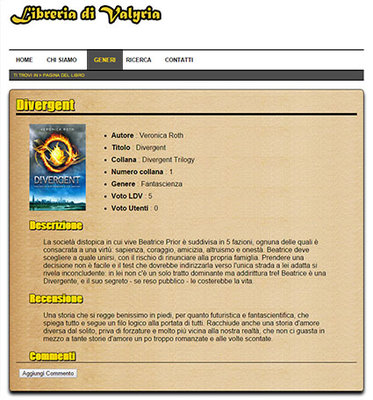
\includegraphics[width=\linewidth]{images/screen/vs_originale.jpg}
\subcaption{Pagina originale (nessun deficit visivo presente)}
\end{minipage}
\hspace{\fill}
\begin{minipage}{0.45\textwidth}
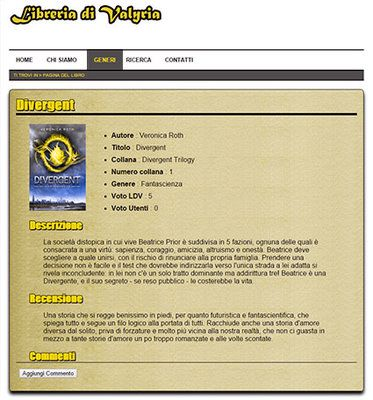
\includegraphics[width=\linewidth]{images/screen/deuteranope.jpg}
\subcaption{Deuteranopia}
\end{minipage}
\vspace*{0.5cm}
\begin{minipage}{0.45\textwidth}
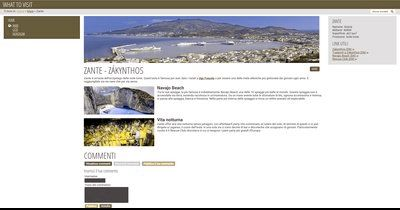
\includegraphics[width=\linewidth]{images/screen/protanope.jpg}
\subcaption{Protanopia}
\end{minipage}
\hspace{\fill}
\begin{minipage}{0.45\textwidth}
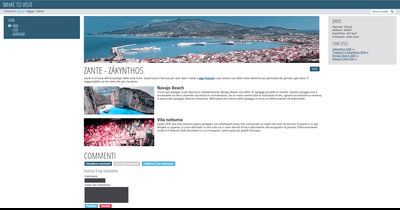
\includegraphics[width=\linewidth]{images/screen/tritanope.jpg}
\subcaption{Tritanopia}
\end{minipage}
\caption{Test con Vischek sulla pagina relativa al singolo libro}\label{multiavp}
\end{figure}

Per quanto riguarda Deuteranopia e Protanopia, la visualizzazione del sito è pressochè identica rispetto all'originale e si differenzia solamente quando si tratta di visualizzare diverse copertine di libri, quando invece si parla di Tritanopia allora si nota un differente modo di vedere gli elementi comuni a tutte le pagine del sito che comunque rimangono accessibili in ogni caso.

\subsection{Visualizzazione in Bianco/Nero}
Abbiamo anche esaminato il sito web con una visualizzazione in scala di grigi notando come alcuni elementi non vengano visualizzati al meglio.

\begin{figure}[H]
\begin{minipage}{0.45\textwidth}
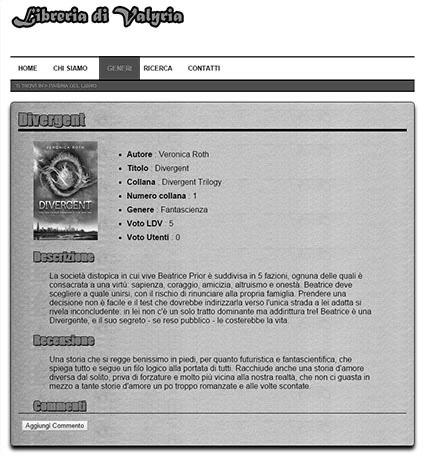
\includegraphics[width=\linewidth]{images/screen/bn_originale.png}
\subcaption{Pagina originale (nessun deficit visivo presente)}
\end{minipage}
\hspace{\fill}
\begin{minipage}{0.45\textwidth}
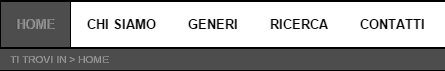
\includegraphics[width=\linewidth]{images/screen/bn_headerbreadcrumb.jpg}
\subcaption{Header e Breadcrumb}
\end{minipage}
\vspace*{0.5cm}
\begin{minipage}{0.45\textwidth}

\includegraphics[width=\linewidth]{images/screen/bn_tornahome.jpg}
\subcaption{Link Visitato in Accedi.html}
\end{minipage}
\hspace{\fill}
\begin{minipage}{0.45\textwidth}
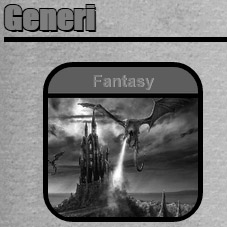
\includegraphics[width=\linewidth]{images/screen/bn_h2etitoli.jpg}
\subcaption{Schede di generi e Titoli}
\end{minipage}
\caption{Errori di visualizzazione nel caso di visione in scala di grigi}\label{multiavp}
\end{figure}

Dalle figure sovrastanti si può notare come vengono visti alcuni elementi quando si effettua una visualizzazione in scala di grigi, e come questi a volte non siano accessibili, come nel caso di link già visitati, in pagine come Accedi o Registrati, Titoli dei Generi, come accade nella pagina di selezione dei generi letterari, o come nel caso di Breadcrumb e Scheda selezionata, in gran parte delle pagine del sito.

\subsection{Fangs}\label{sec:fangs} %DONE
\textit{Fangs} è un'estensione per i browser che consente di visualizzare un
sito nello stesso modo in cui verrebbe visualizzato da uno screen reader,
fornendo il testo come sarebbe letto da questo dispositivo, la lista delle
intestazioni e la lista dei link presenti nella pagina.

In sintesi, come principali problemi vengono individuati:
\begin{itemize}
\item Le parole straniere vengono lette in italiano;
\item A volte i numeri sono scritti in numero; ciò vuol dire che se l'utente
ha la lingua di default del computer/browser impostata su inglese (come nel
caso di un verificatore) si hanno frasi come ``\textit{La società distopica in
cui vive Beatrice Prior è suddivisa in five fazioni}", mentre in casi simili
un numero dovrebbe essere scritto per esteso;
\item Si vedono i nomi dei file delle immagini anzichè un testo alternativo;
\item Quando presente, il testo delle immagini spesso trasmette poca
informazione, ridondando semplicemente il titolo anzichè rimanere vuoto
(soluzione preferibile alla ridondanza);
\item Le abbreviazioni non vengono estese, diventando potenzialmente
incomprensibili.
\end{itemize}

\subsection{Lynx}\label{sec:lynx} %DONE
Le pagine del sito sono state anche navigate tramite il browser testuale
\textit{Lynx}.

Come principale difetto, non è possibile effettuare l'accesso a funzioni come
accesso e registrazione, poichè tutti i pulsanti hanno la sottomissione
dell'input gestita tramite JavaScript, quindi per testare tutte le pagine, si è
provveduto a fare una copia dei file una volta loggati tramite browser e poi
ogni pagina è stata aperta con Lynx.

Gli errori rilevati sono gli stessi discussi nelle altre sezioni.

\subsection{Performance}
Per terminare la fase di testing sono state eseguite, con strumenti
automatici, una serie di verifiche riguardo le performance del sito.

Ci siamo avvalsi di tool online\footnote{\texttt{https://developers.google.com/speed/pagespeed/insights/}, \texttt{http://www.webpagetest.org/},
\texttt{http://gtmetrix.com/}} che analizzano in profondità le pagine HTML
fornite e restituiscono: consigli di ottimizzazione, scale di punteggi per ogni
aspetto del sito e una serie di statistiche che vedremo in dettaglio.\footnote{NB: Per poter utilizzare i tester il sito è stato ``hostato" sulla piattaforma GitHub Pages, come scritto all'inizio di questa sezione}

Al fine di uniformare i risultati raccolti da questi strumenti abbiamo deciso
di mostrare solo alcune delle pagine analizzate, una per ogni livello
gerarchico.
In particolare le più significative per ogni livello (\texttt{homepage.html},
\texttt{citta.html},\texttt{london.html}) hanno dato i seguenti esiti:

\begin{figure}[h]
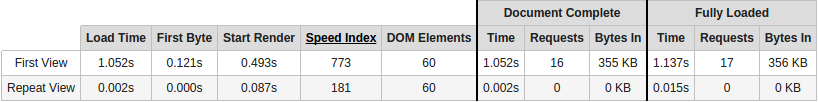
\includegraphics[width=\linewidth]{images/performance/webpagetest/home.png}
\caption{Homepage: tempi di caricamento}
\label{fig:tempiHome}
\end{figure}

\begin{figure}[h]
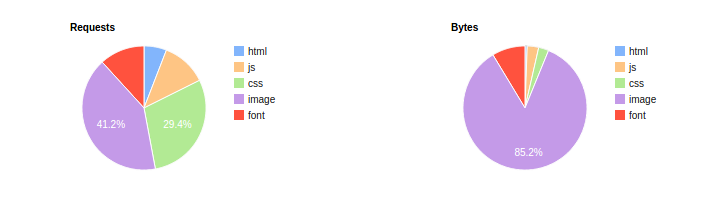
\includegraphics[width=\linewidth]{images/performance/webpagetest/home-graph.png}
\caption{Homepage: Grafico a 'torta' dei tempi di caricamento}
\end{figure}

In homepage si nota la prevalenza del flusso delle immagini, come evidenziato
in fig.\ref{fig:tempiHome}, dal diagramma circolare delle richieste e della
quantità di dati trasmessi dal server.

Come è facile aspettarsi, le immagini occupano in termini di peso la maggior
parte del sito e le richieste per il loro recupero rappresentano più del 40\%
delle richieste totali.


Lo stesso esito è stato conseguito in \texttt{citta.html} e
\texttt{london.html} (fig.\ref{fig:tempiOther}), sebbene \texttt{citta.html}
sia leggermente più pesante dal momento che viene fatto un uso più intenso dei
fogli di stile.

Dopo aver eseguito i test sulle stesse pagine per 3 volte abbiamo stimato che il tempo medio di caricamento complessivo si aggira intorno ai 1400ms.

I test sulla velocità di caricamento sono stati effettuati su di un client residente negli Stati Uniti avente browser Chrome.


\begin{figure}[h]
\begin{minipage}{0.45\textwidth}
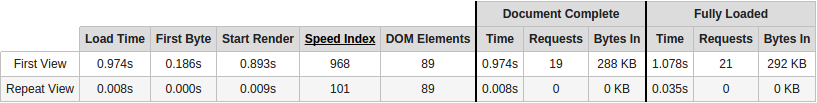
\includegraphics[width=\linewidth]{images/performance/webpagetest/citta.png}
\subcaption{\textit{citta.htm}l: tempi di caricamento}
\end{minipage}
\hspace{\fill}
\vspace*{0.5cm}
\begin{minipage}{0.45\textwidth}

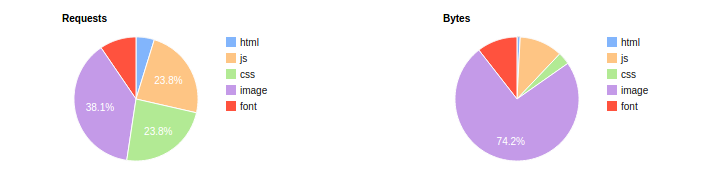
\includegraphics[width=\linewidth]{images/performance/webpagetest/citta-graph.png}
\subcaption{\texttt{citta.html}: grafico a 'torta'}
\end{minipage}

\begin{minipage}{0.45\textwidth}
\vspace*{0.5cm}
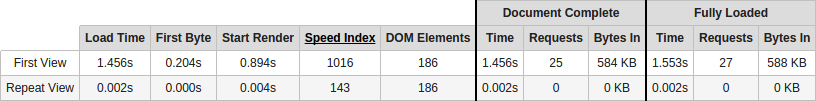
\includegraphics[width=\linewidth]{images/performance/webpagetest/london.png}
\subcaption{\texttt{london.html}: tempi di caricamento}
\end{minipage}
\hspace{\fill}
\vspace*{0.5cm}
\begin{minipage}{0.45\textwidth}

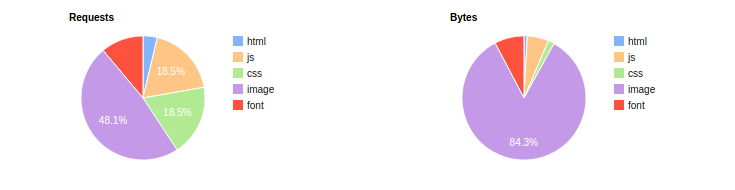
\includegraphics[width=\linewidth]{images/performance/webpagetest/london-graph.png}
\subcaption{\textit{london.html}: grafico a 'torta'}
\end{minipage}
\caption{Performance in \texttt{citta.html} e \texttt{london.html}}\label{multiavp}
\label{fig:tempiOther}
\end{figure}

Complessivamente il sito ha totalizzato una media di 71 punti su 100 totali in Google PageSpeed Insights.

Le ottimizzazioni suggerite per aumentarne il punteggio andavano per lo più
contro standard W3C e/o compatibilità con i browser più obsoleti. Abbiamo
quindi deciso di adottare le soluzioni che permettessero di mantenere
l'accessibilità del sito, cercando di alleggerirlo con piccoli accorgimenti
(e.g. minificazione della libreria Require.js, immagini a risoluzione
inferiore mantenendo una certa qualità di fondo, ecc.) trovando un buon
compromesso tra velocità di caricamento e compatibilità con più browser.